\chapter{Multi-Robot Lattice Formation Problem}
\label{chp:mrf}

In this chapter, we address a multi-robot lattice formation problem.
%
Consider a set of robots, in which each
robot can only use local information.
We focus on a problem in which the robots want to form an arbitrary lattice patterns autonomously.


The remaining sections of this chapter are organized as follows. 
%
Section~\ref{sec:related-mrf} gives a summary of related work on the multi-robot formation problems.
%
Specifically, we review the work focusing on solving the problems in a distributed manner. 
%
Section~\ref{sec:robot-model} illustrates the robot model we have used in this multi-robot lattice formation problem.
%
Section~\ref{sec:latt-graph} introduces the graph concepts we have used to represent the output lattice pattern in our problem formulation, and to analyze the robots' communication activities. 
%
Section~\ref{sec:mrf-eval} defines two criteria we have used to evaluate our formation algorithms.
%
The concepts of robot model, the lattice graph, and the evaluation criteria are commonly used by two different formation algorithms in Chapter~\ref{chp:mrf1} and Chapter~\ref{chp:mrf2}.

%\clearpage
\section{Related Work}
\label{sec:related-mrf}

Distributed solutions are powerful and efficient for many applications of multi-robot systems,
such as deploying multiple robots or large-scale sensor networks to execute searching or sensing tasks. 
%
Previously, a lot of work has been done on the multi-robot lattice formation
problem using distributed methods. 
%
Fujibayashi, Murata, Sugawara and Yamamura proposed a probabilistic control algorithm to generate the triangular lattice pattern~\cite{FujMurSugYam02}. 
%
Hanada, Lee and Chong constructed an algorithm to form separated triangular lattices and then reunify
them as a whole in an environment with obstacles~\cite{HanLeeCho07}.  
%
Notably, approaches using artificial virtual forces, such as the physicomimetics framework (PF), 
were well-studied in forming repeated lattice patterns, such as
triangular, square, and hexagonal lattices~\cite{FujMurSugYam02, HanLeeCho07,
  SpeSpeHamHei04, SpeHeiZar05, MarPay2005, NavPugMarMat09, LeeBecFekKroMcL14,
  PraLiMcLu12, MulMonBarRem13}. 
%  
Robots can quickly form specific lattice patterns using attractive or repulsive forces to adjust their positions based on only measurements of range and bearing to nearby robots.  
%
W. Spears, D. Spears, Heil, Zarzhitsky, and Hamann discussed swarm intelligence and applied PF-based
methods to systems with multiple particle robots to form hexagonal lattices~\cite{SpeSpeHamHei04}.  
%
Martinson and Payton extended the PF-based algorithm by adding an extra alignment step before applying the virtual force among robots.  
%
The robots first move to parallel lines using compasses and then form a square lattice using 
the virtual force, without suffering from local minima~\cite{MarPay2005}.  
%
Navarro, Pugh, Martinoli, and Mat{\'\i}a implemented a PF-based algorithm as a finite state machine, 
so that robots without holonomic assumption can form the triangular lattice~\cite{NavPugMarMat09}.  
%
Based on the PF-based approach that is used for the triangular formation, 
Mullen, Monekosso, Barman, and Remagnino designed a cooperative formation control strategy to form hexagonal lattices. 
%
Their robots coordinate with each other to determine the centroids of hexagonal cells and place
virtual robot nodes in those positions to avoid local minima~\cite{MulMonBarRem13}. 
%
Prabhu, Li, and McLurkin designed a local error correction algorithm to detect and correct misplacements in a hexagonal lattice formation using artificial forces~\cite{PraLiMcLu12}.


Nevertheless, both probabilistic control formation algorithms 
and virtual-force-based methods have a common limitation: 
they are used only to form exclusively one specific lattice
pattern which is known to the algorithm designer.


In contrast, Chaimowicz, Michael, and Kumar addressed a decentralized control
framework to place holonomic robots in different shapes based on their local
state feedback and sensing~\cite{ChaMicKum05}. 
%
Since the control law is given by the gradient of the implicit function which is represented by the zero isocontour of a 3D surface, the major limitation of this approach is concerned with local minima. 
%
Ikemoto, Hasegawa, Fukuda, and Matsuda described a gradual pattern formation approach for homogeneous robots to form miscellaneous geometric shapes.
They proposed a Turing morphogenetic function~\cite{Turing37} to generate patterns based on local information~\cite{IkeHasFukMat05}. 
%
Under this approach, the final pattern is always generated from a circle pattern formed by robots in the
previous step. Thus, it is difficult to use this approach to form any repeated
pattern.


In contrast to the above-mentioned methods, our algorithm accepts a graph
representation of desired lattice pattern as part of its input.


Another trend of related work solves multi-robot formation problems using task
assignment approaches. 
%
Smith and Bullo demonstrated a provably-correct geometric target assignment method to allocate robots to distinct target locations~\cite{SmiBul07}.  
%
Michael, Zavlanos, Kumar, and Pappas proposed a distributed control approach for non-holonomic robots performing different formation tasks.  
%
They introduced a market-based coordination strategy in which each robot determines its destination by bidding for task assignments~\cite{MicZavKumPap08}.  
%
Both algorithms require only local communication. 
%
One limitation is that these algorithms do not guarantee the optimal assignment. 
%
Moreover, task-assignment-based algorithms require the robots to have knowledge of all the tasks in advance.  
%
MacDonald extended the work of Michael et al.~\cite{MicZavKumPap08} by assuming the robots can acquire their
tasks online.  
%
In MacDonald's thesis, he applied the iterative closest point algorithm~\cite{RusLev01} in order to match a set of
robot positions to the set of model data of the target formations~\cite{Mac11}.  
%
The author showed finally the target formations were asymptotically stable using his improved method if each robot knows relative positions of all other robots, but the algorithm will not converge if
some robots lose communication with other robots~\cite{Mac11}.


Alonso-Mora, Breitenmoser, Rufli, Siegwart, and Beardsley proposed a control
strategy to form arbitrary patterns, in which the goal positions for the final
patterns are first generated via a Voronoi partition, after which a task
assignment algorithm was performed to coordinate the robots~\cite{AloBreRufSieBea11}. 
%
However, the authors conducted centralized task assignment to compute an optimal formation, and used distributed controllers only for local collision avoidance.  
%
This approach does not seem applicable if only local information is available for each robot.  
%
Liu and Shell discussed a special gradual formation problem called ``formation morphing,'' 
that is, as the formation is gradually deformed in places, the formation changes but the major
pattern remains unchanged~\cite{LiuShe12}. 
%
They addressed this morphing problem in terms of the task assignment problem incorporated with the graph matching problem~\cite{Lov86}. 
%
The authors represented the robots routing trajectories using a Euclidean graph.  
%
These trajectories are projected from the augmenting paths in the bipartite graph 
so that an optimal formation morphing can be achieved~\cite{LiuShe12}.

The primary limitation common to all of these task-assignment-based algorithms
is that each robot needs to know its global coordinates and all the target
positions in the global sense. 
%
Hence, they are expensive and difficult to apply directly to a large-scale multi-robot system. 
%
Our algorithms offer each robot a way to represent the desired formation using a graph.
%
Different from the Euclidean graph in Liu and Shell's work~\cite{LiuShe12},
we assign the rigid body transformation to each graph edge so that the graph
reflects both location and orientation relationship between two vertices. 
%
Consequently, in Chapter~\ref{chp:mrf1}, we describe a primary algorithm enabling robots to
distribute the computation of task assignments and destinations using local sensing
and communication in its body coordinate frame.


We have observed that the disconnection of the robots' communication
graph has a major negative impact on the final formation quality in our
primary algorithm~\cite{SonOKa14}. 
%
Therefore, we have designed a novel motion plan to enforce the connectivity of robots' communication.
%motivated by a multi-robot recovery problem.
%
In Chapter~\ref{chp:mrf2}, we also have contributed a method to maintain a global
spanning tree constructed from local communication, 
without using the distributed task assignment idea.


Habibi and McLurkin presented an approach to build a maximum-leaf
spanning tree to guarantee the connectivity of robots' network
communication~\cite{HabMcL14}.
%
In Habibi's work, the spanning tree, rooted at the goal location where
all the robots should be recovered, provided each robot a path to the
goal. 
%
Moreover, only the leaves of the spanning tree were allowed to move during
the recovery, whereas the internal nodes remained motionless as a
navigation guide to lead the robots back to the root.
%
We have developed a different strategy to construct a spanning tree of the communication
graph. 
%
In contrast to their approach, which drives the maximum number of leaves to
one goal, our plan is, in our spanning tree, 
relocating only one robot to a specified goal position, 
while generating small but
necessary movements of the others to preserve connectivity.


%\clearpage
\section{Robot Model}
\label{sec:robot-model}
We consider a collection of $n$ identical robots $R = \{r_1, \ldots, r_n \}$ moving through an obstacle-free plane. 
%
We assign each robot a unique, comparable \textbf{identification (ID) number} $\id(r)$, 
so that any pair of two robots can decide the numerical order of their IDs.
%
We describe the robot model as following.
\begin{enumerate}
\item Robot pose and coordinate frames: For a robot $r_i$, denote its pose using
  $p_i = (x_i, y_i, \theta_i)$. A pose $p_i$ consists of a position and an
  orientation, expressed in an arbitrary but fixed global coordinate frame for
  modeling purposes. Write the pose of $r_i$ at time $t$ as $p_i(t)$.  Also
  define a body frame attached to each robot, in which the robot is always at
  the origin, facing along the positive $x$-axis.  Let $\Tr(r_i)$ denote the $3
  \times 3$ homogeneous matrix representing the rigid body transformation from
  the body frame of $r_i$ to the global frame:
  \begin{equation}
    \label{eq:trans}
    \Tr(r_i) =  \begin{bmatrix}
      \cos{\theta_i} & - \sin{\theta_i} & x_i\\
      \sin{\theta_i} & \cos{\theta_i} & y_i \\
      0 & 0 & 1\\
    \end{bmatrix}.
  \end{equation}
  The robots have no access to the information in the global frame,
  instead, only the information in their body frames are used. 
  Denote the local pose of robot $r_j$ in the body frame of robot $r_i$ using
  $p_j^{(i)} = (x_j^{(i)}, y_j^{(i)}, \theta_j^{(i)})$.
\item Robot motion: Assume each robot can move forward with maximum
  linear velocity $v_{max}$ and can rotate in place with unbounded
  angular velocity.
\item Robot neighbors: Assume each robot can sense and
  communicate with other robots within a short distance from its
  position, called the robot's \textit{range} and written as $\range$.
  The other robots within that range are called the \textit{neighbors}
  of that robot.
\item Robot observations: Assume the sensors of each robot can generate
  a collection of observations consisting of neighbors' IDs and poses
  in view of robot's body frame.
\item Robot messages: Each robot broadcasts messages to its neighbors
  containing information used by robots to make decisions (details are
  described in Chapter~\ref{chp:mrf1} and Chapter~\ref{chp:mrf2}). 
\end{enumerate}

We assume that the sensing and communication occur in discrete time steps. 

To analyze communication in the entire robot system, we use a graph structure to represent the relevant information.

\begin{defn}
  Given a set of robots $R =\{r_1, ..., r_n\}$, the \textbf{communication
  graph} is a graph in which each vertex is a robot, and there exists an
  undirected edge between two vertices if corresponding robots are neighbors.
\end{defn}

In the communication graph, if there exists any path composed of edges between two vertices, we use the term
\textbf{steps} to denote the number of edges in the shortest path between
them.

Two assumptions here, namely synchronous clocks and unbounded angular velocity, 
would of course be quite difficult to realize in a practical multi-robot system. 
%
These assumptions are used to simplify the connectivity analysis in Lemma~\ref{lem:boundedrange} in Chapter~\ref{chp:mrf1} and Chapter~\ref{chp:mrf2}, 
and are not crucial to the correctness of the algorithm.


%\clearpage
\section{Lattice Graph}
\label{sec:latt-graph}
One core contribution is that we have introduced a graph definition to represent a lattice pattern.
%
\begin{defn}
  \label{def:latticegraph}
  A \textbf{lattice graph} is a strongly connected directed multigraph in which
  each edge $e$ is labeled with a rigid body transformation $\Tr(e)$ and each
  $\edge{u}{\Tr(e)}{w}$ has an inverse edge $\edge{w}{\Tr(e)^{-1}}{u}$.
\end{defn}

The intuition is, we want each robot to be associated with one lattice graph vertex, 
and the outgoing edges of that vertex will correspond to the relative poses of that robot's neighbors when the lattice is correctly formed.
%
Figure~\ref{fig:edgetrans} shows a simple example in which the positions of two
robots satisfy the given lattice graph. 
A robot with the role $w$ is
at pose $(l\cos{\alpha}, l\sin{\alpha}, \beta-\alpha)$ relative a robot with the role of
$u$. Here the role functions are: $f(r_i) = u, f(r_j) = w$.


The lattice graph in Figure~\ref{fig:sq} represents a repeating square lattice pattern, 
in which one node has four outgoing edges connecting to itself. 
%
The graph also reflects local neighborhood relationships:
%
Every pair of poses satisfying the rigid-body transformation of an outgoing edge is a component of the repeating square pattern.
%
Figure~\ref{fig:hex} shows an example of the lattice graph used to represent a
repeating hexagon lattice, in which there are two nodes, each one has three outgoing edges connecting to the other one. 
%
To show that our algorithm is sufficient for complicated patterns, 
we have designed a lattice graph representing a repeating octagon-square lattice pattern shown in Figure~\ref{fig:octagonsquare}.
%

%%%%%%%%%%%%%%%%%%%%%%%%%%%%%%%%%%%%%%%%
\begin{figure}
  \centering
   \begin{minipage}[b]{0.4\linewidth}
    \centering
    \begin{tikzpicture}[scale=1.2]
      \tikzstyle{every state}=[fill=red!50, draw=none]
      \node[state, scale=0.6] (A) at (0, 1)  {\large{$u$}};
      \node[state, scale=0.6] (B) at (3, 1)  {\large{$w$}};
      \draw[arc] (A) to[out=60, in=150] (B);
      \draw[arc] (B) to[out=-120, in=-30] (A);
      %\node[] at (1.5, 2) {$e_v^w$};
      \node[] at (1.5, 2.25) {\footnotesize{$\left(l\cos{\alpha}, l\sin{\alpha}, \beta-\alpha\right)$}};
      %\node[] at (1.5, 0) {$e_w^v$};
      \node[] at (1.5, -0.25) {\footnotesize{$\left(-l\cos{\alpha}, l\sin{\alpha}, \alpha-\beta\right)$}};
    \end{tikzpicture}
  \end{minipage}
  \begin{minipage}[b]{0.5\linewidth}
    \centering
    \begin{tikzpicture}[scale=1.2]
      \draw[fill=red] (2,2) -- (1.69, 1.74) -- (2.12,2.47) -- (2.16,1.64) -- cycle;
      \draw[fill=blue] (0,0) -- (-0.136,-0.375) -- (-0.13, 0.48) -- (0.35, -0.2) -- cycle;
      \draw[post] (0,0) -- (1.7,1.7);
      \draw[dashed](2, 2) -- (2.5, 2.5);
      \draw[dashed](2, 2) -- (2.26,2.97);
      \draw[dashed](0, 0) -- (-0.26, 0.97);
      \draw[dashed](0.5, -0.5) -- (0, 0);
      \coordinate (A) at (-0.14, 0.53);
      \coordinate (B) at (0.45, 0.45);
      \draw[arc] (A) to[out=45, in=135] (B);
      \coordinate (C) at (2.4, 2.4);
      \coordinate (D) at (2.155, 2.58);
      \draw[arc] (C) to[out=135, in=-30] (D);
      \node[] at (2.5, 2.7) {$\beta$};
      \node[] at (0.2, 0.9) {$\alpha$};
      \node[] at (-0.5, 0) {$r_i$};
      \node[] at (1.7, 2.2) {$r_j$};
      \node[] at (0.75, 1.25) {$e_u^w$};
      \coordinate (X2) at (0.25, -0.25);
      \coordinate (X1) at (1, 0.5);
      \draw[edge] (X1) -- (X2);
      \node[] at (1.25, 0.75) {$l$};
      \coordinate (Y1) at (1.5, 1);
      \coordinate (Y2) at (2.25, 1.75);
      \draw[edge] (Y1) -- (Y2);
      \draw[dashed] (2,2) -- (2.5, 1.5);
    \end{tikzpicture}
  \end{minipage}
  \caption{[left] Two nodes $u, w$ in a lattice graph.  The edge from $u$ to
    $w$ reflects the rigid body transformation between the two: a robot in role $w$ is at pose
    $(l\cos{\alpha}, l\sin{\alpha}, \beta-\alpha)$ relative a robot in role
    $u$.  [right] Poses of robots $r_i$ and $r_j$ that satisfy this lattice graph, 
    with role functions $f(r_i) = v, f(r_j) = w$.
    }

  \label{fig:edgetrans}
\end{figure}
%%%%%%%%%%%%%%%%%%%%%%%%%%%%%%%%%%%%%%
%TODO Penrose tiling 

\begin{defn}
\label{def:selfconsist}
  Given a lattice graph $G=(V, E)$ and a set of robots
    $R = \{ r_1, \ldots, r_n \}$,
  we say that $R$ \textbf{satisfies} $G$ if there exists a function
    $f: R \rightarrow V$
  that preserves the neighborhood structure of $G$.
  %
  Specifically, for any $i$ and $j$, if $r_i$ and $r_j$ are neighbors, 
  there must exist an edge
  $e_u^w: \edge{f(r_i)}{}{f(r_j)}$ in $E$, such that 
      $f(r_i) = u$,
      $f(r_j) = w$, and $\Tr(r_j) = \Tr(r_i) \Tr(e_{u}^w)$.
\end{defn}

%%%%%%%%%%%%%%%%%%%%%%%%%%%%%%%%%%%%%%
\begin{figure}
    \centering
    \begin{minipage}[b]{0.45\linewidth}
        \centering
        %% \begin{tikzpicture}[->,>=stealth',shorten >=5pt,auto,node distance=1cm]
%%   \tikzstyle{every state}=[fill=orange!50, draw=none]
%%   \node[state, scale=0.6] (A)         {$0$};
%%   \path (A) edge [loop above] node {\footnotesize{\left(0, 1, 0\right)}} (A)
%%   edge [loop left]  node {\footnotesize{\left(-1, 0, 0\right)}} (A)
%%   edge [loop below] node {\footnotesize{\left(0, -1, 0\right)}} (A)
%%   edge [loop right] node {\footnotesize{\left(1, 0, 0\right)}} (A);
%% \end{tikzpicture}
%\caption{The lattice graph representing a repeated square pattern.}
\begin{tikzpicture}[->,>=stealth',shorten >=5pt,auto,node distance=1cm]
  \tikzstyle{every state}=[fill=red!50, draw=none]
  \node[state, scale=0.7] (A)         {$0$};
  \path (A) edge [loop above] node {\footnotesize{(0,1,0)}} (A)
  edge [loop left]  node {\footnotesize{(-1,0,0)}} (A)
  edge [loop below] node {\footnotesize{(0,-1,0)}} (A)
  edge [loop right] node {\footnotesize{(1,0,0)}} (A);
\end{tikzpicture}

    \end{minipage}
    \begin{minipage}[b]{0.45\linewidth}
        \centering
        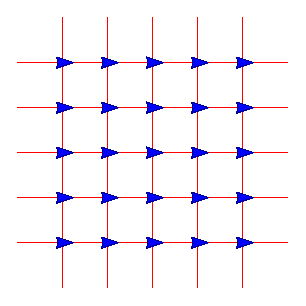
\includegraphics[trim=0.5cm 0.5cm 0.5cm 0.5cm, clip=true]{figs/sq-lat}
    \end{minipage}
    \caption{[left] A lattice graph representing a repeated square
    pattern. There is one node with four outgoing edges connecting to
    itself. Here the edge length is $1$. For a robot playing the role
    of this node, its neighbors should be in locations $(1, 0), (0,
    -1), (-1, 0)$ and $(0, 1)$, with the same orientation. [right]
    A repeated square lattice pattern represented by the left
    graph.}
    \label{fig:sq}
\end{figure}
%%%%%%%%%%%%%%%%%%%%%%%%%%%%%%%%%%%%%%
\begin{figure}
    \centering
    \begin{minipage}[b]{0.45\linewidth}
        \centering
        
    \begin{tikzpicture}[->,>=stealth',shorten >=5pt,auto,node distance=3cm]
      \tikzstyle{every state}=[draw=none]
      \node[state, scale=0.7, fill=red!50] (A) at (0,0)    {$0$};
      \node[state, scale=0.7, fill=blue!50] (B) at (3,0)  {$1$};
      \path (A) edge [bend left=10] node {\scriptsize{(0, 40,0)}} (B)
            (A) edge [bend left=45] node {\scriptsize{(-35,-20,0)}} (B)
            (A) edge [bend left=90] node {\scriptsize{(35,-20,0)}} (B)
            (B) edge [bend left=10] node {\scriptsize{(-40,0,0)}} (A)
            (B) edge [bend left=45] node {\scriptsize{(35,20,0)}} (A)
            (B) edge [bend left=90] node {\scriptsize{(-35,20,0)}} (A);
    \end{tikzpicture}
  
    \end{minipage}
    \begin{minipage}[b]{0.45\linewidth}
        \centering
        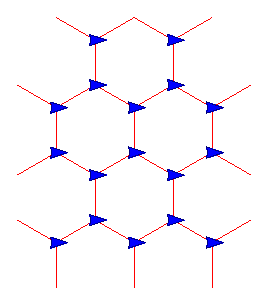
\includegraphics[scale=0.85]{figs/hex-lat}
    \end{minipage}
    \caption{[left] A lattice graph representing a repeating hexagon lattice pattern on the right. 
    In the graph, the edge length is $40$. 
    For a robot playing the role vertex $0$, its neighbors should be in locations $(35, -20), (-35, -20)$ and $(0, 40)$ with the same headings, and its neighbors should play the role vertex $1$ which has an outgoing edge to vertex $0$. 
    [right] A repeating hexagon lattice pattern represented by the left graph.}
    \label{fig:hex}
\end{figure}
%%%%%%%%%%%%%%%%%%%%%%%%%%%%%%%%%%%%%%
\begin{figure}
    \centering
    \begin{minipage}[b]{0.45\linewidth}
        \centering
        \begin{tikzpicture}[->,>=stealth',shorten >=5pt,auto,node distance=1.5cm]
    \tikzstyle{every state}=[fill=red!50, draw=none]
            %                  D
            %      C      A 
            % 
            %             B
        \node[state, scale=0.7] (A) at (0,0)    {$0$};
        \node[state, scale=0.7, fill=cyan] (B) at (0,-2)  {$1$};
        \node[state, scale=0.7, fill=blue!50] (C) at (-2,0) {$2$};
        \node[state, scale=0.7, fill=orange] (D) at (1,1) {$4$};
        \path (A) edge (B)% node {\scriptsize{Tr(0, -40)}} (B)
              (A) edge (C) %node {\scriptsize{Tr(-40, 0)}} (C)
              (A) edge (D); %node {\scriptsize{Tr(28,28)}}  (D);
        \path (B) edge [bend left=10] (A)
              (B) edge (D) % node {\scriptsize{Tr(-40,0)}}  (D); 
              (B) edge (C);% node {\scriptsize{Tr(-28,28)}} (C);
        \path (C) edge [bend right=30] (B)
              (C) edge [bend left=10] (A)
              (C) edge [bend left=30] (D);
        \path (D) edge [bend left=30] (B)
              (D) edge [bend right=10] (A)
              (D) edge (C);
\end{tikzpicture}
    \end{minipage}
    \begin{minipage}[b]{0.45\linewidth}
        \centering
        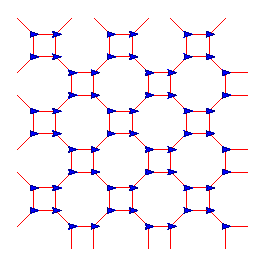
\includegraphics[scale=0.95]{figs/octsq-lat}
    \end{minipage}
    \caption{[left] A lattice graph representing a repeating octagon-square lattice pattern on the right (for simplicity, we do not show the edges' transformations). [right] A repeating octagon-square lattice pattern represented by the left graph.}
    \label{fig:octagonsquare}
\end{figure}
%%%%%%%%%%%%%%%%%%%%%%%%%%%%%%%%%%%%%%

%%%%%%%%%%%%%%%%%%%%%%%%%%%%%%%%%%%%%%
\begin{figure}
    \centering
    \begin{minipage}[b]{0.45\linewidth}
        \centering
        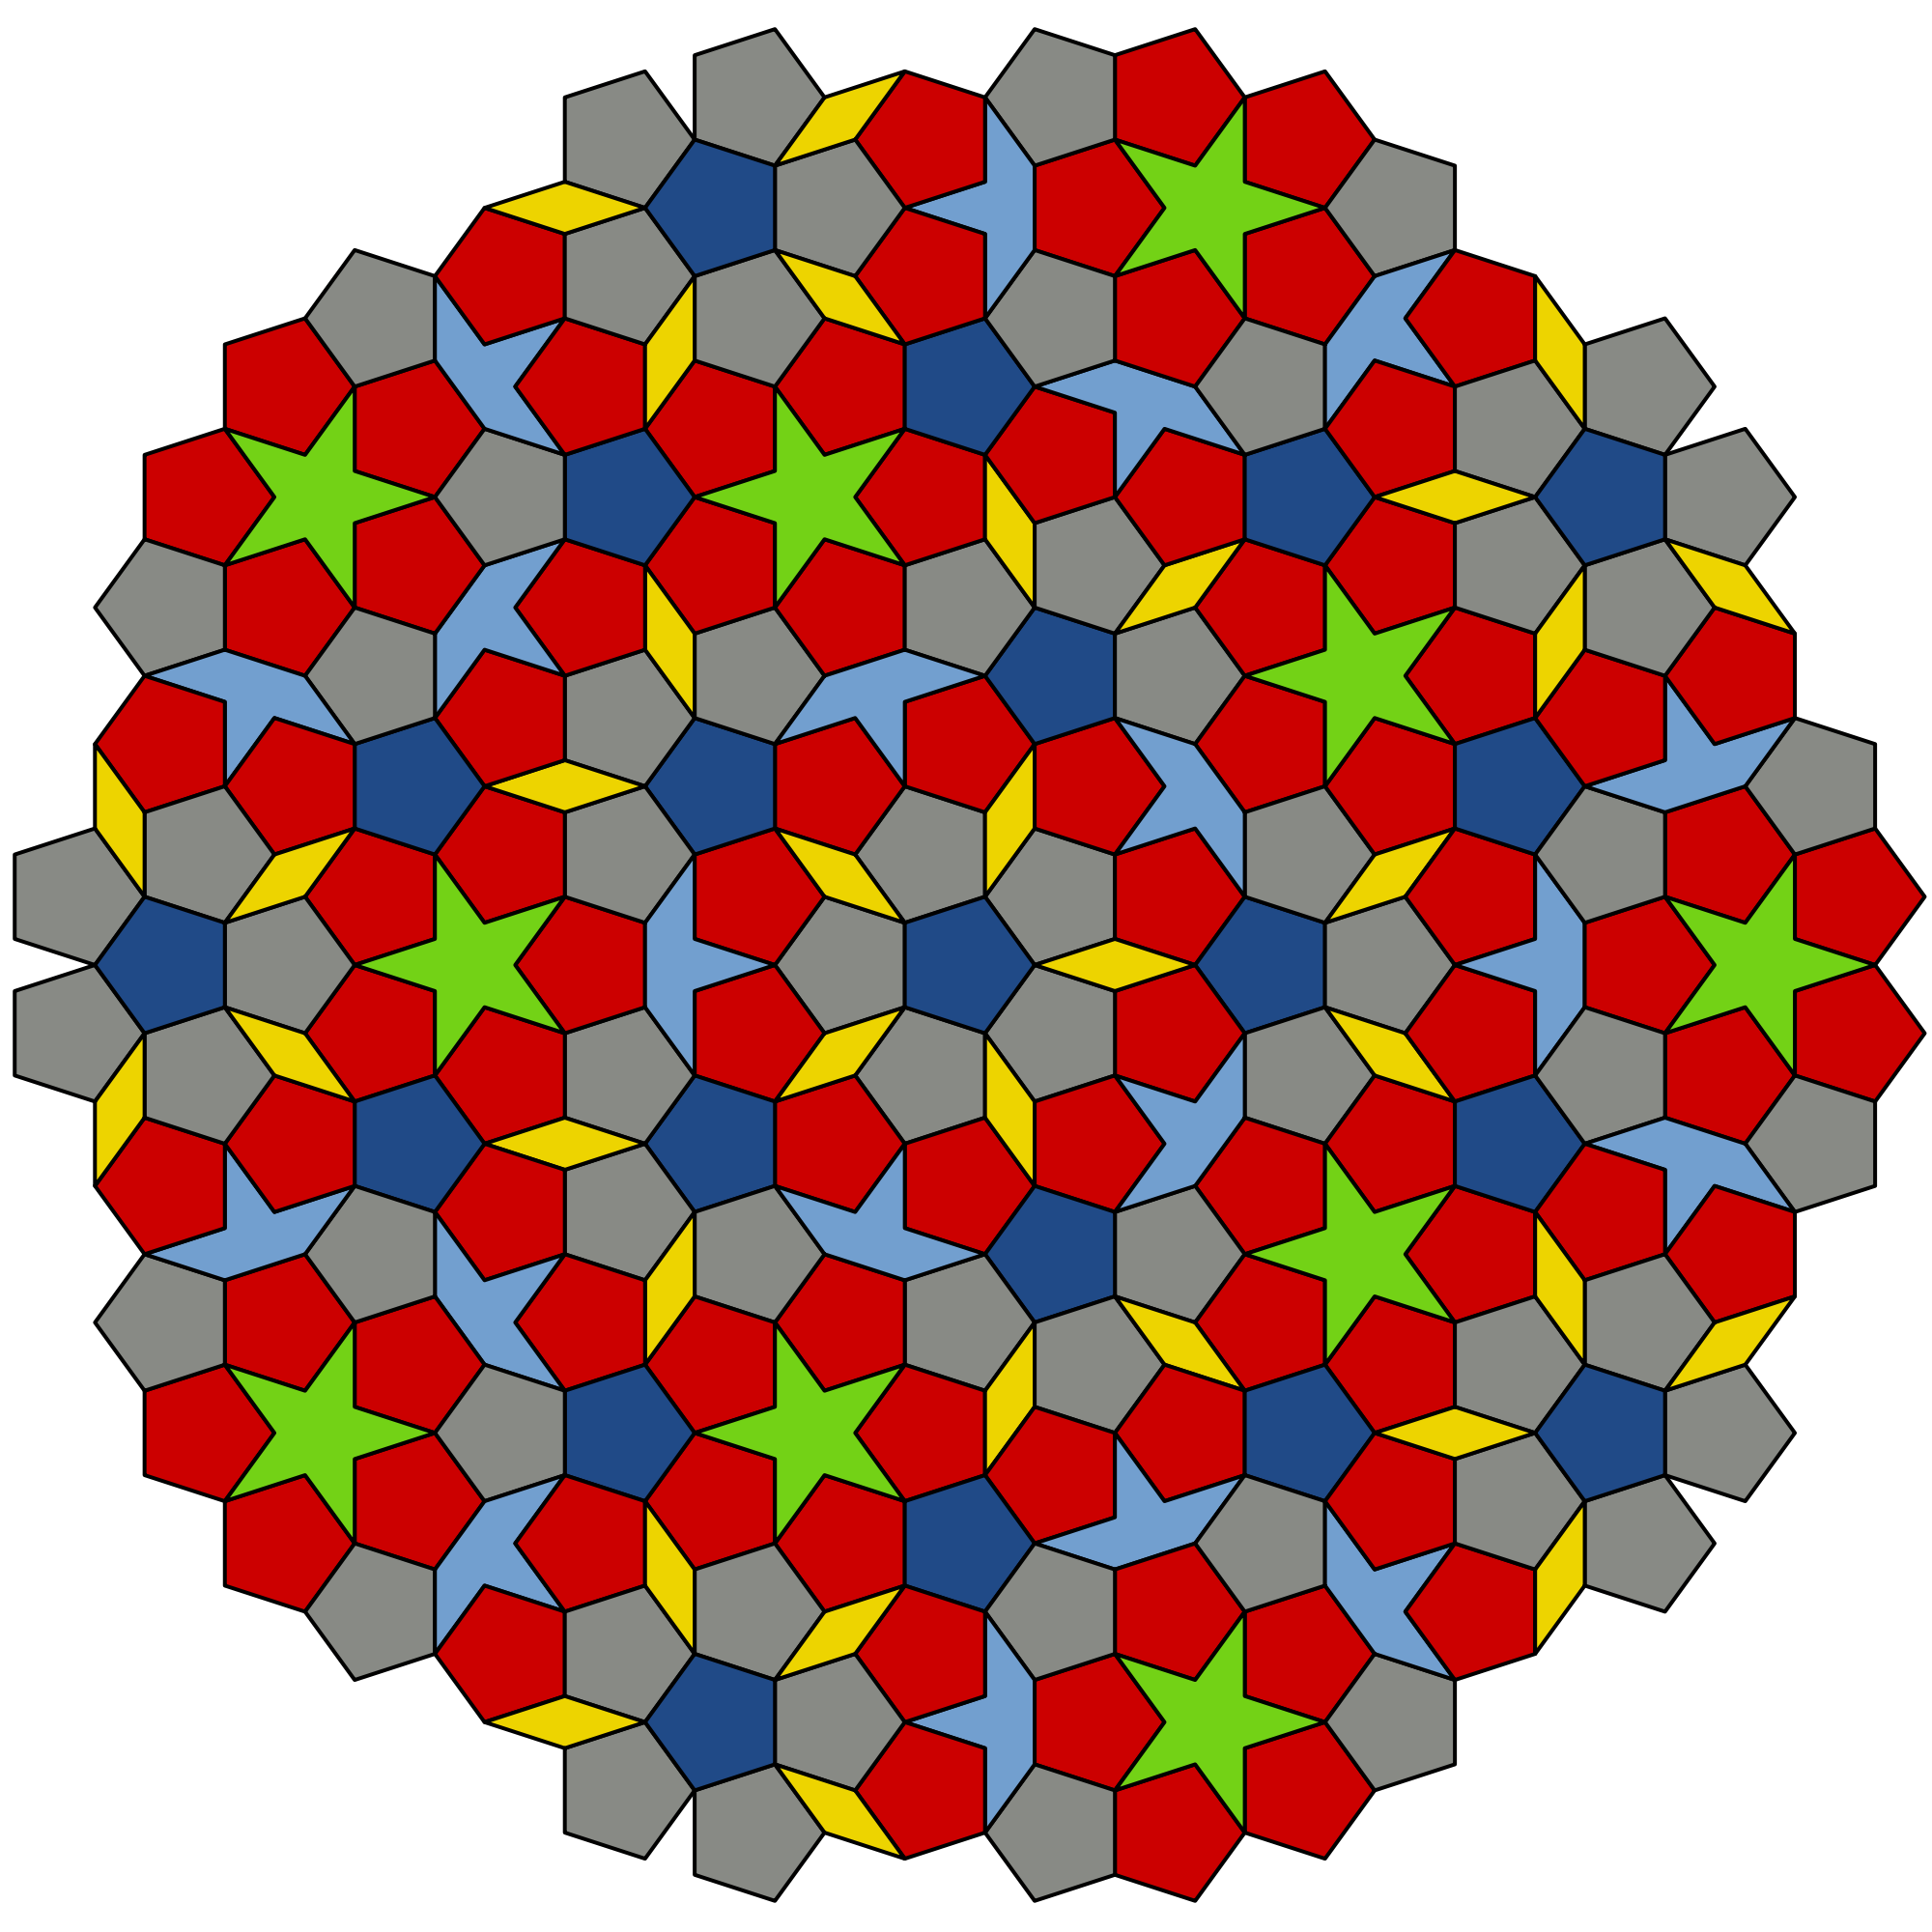
\includegraphics[width=0.9\textwidth]{figs/Penrose_Tiling.png}
    \end{minipage}
    \begin{minipage}[b]{0.45\linewidth}
        \centering
        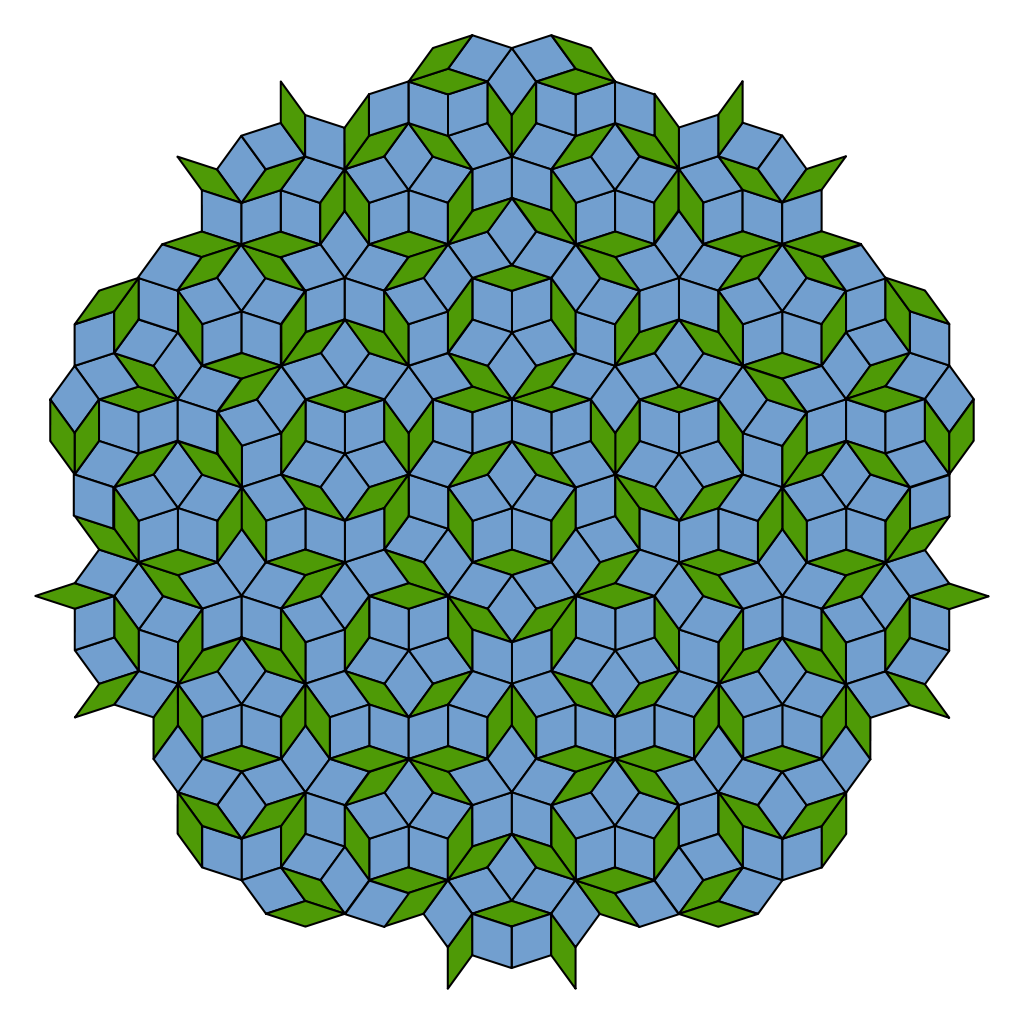
\includegraphics[width=0.9\textwidth]{figs/Penrose_Tiling2.png}
    \end{minipage}
    \caption{Two penrose tiling patterns.}
    \label{fig:penrose}
\end{figure}
%%%%%%%%%%%%%%%%%%%%%%%%%%%%%%%%%%%%%%

The lattice graph is suitable for representing repeated patterns, but not the non-periodic patterns, 
such as the Penrose tiles~\cite{Pen79, Gum96}. 
(Figure~\ref{fig:penrose} shows two Penrose tiles, which are pairs of tiles placed aperiodically, called ``kite'' and ``dart''.)


\subsection{Lattice Graph Constraint}
The graph definition of a lattice may describe a geometric pattern that contradicts itself. 
To guarantee a pattern is represented properly using a lattice graph, we define a constraint, termed ``self-consistent'', for a lattice graph, so that the represented pattern will not contradict itself by forcing pairs of robots to be mutual neighbors, with roles that are not adjacent in the lattice graph. 
%
Figure~\ref{fig:self-consistent-graph} shows a comparison between a simple
lattice graph that is not self-consistent with one that is self-consistent.



\begin{defn}
  \label{def:selfconsistent}
  Given a range $\range > 0$, call a lattice graph \textit{self-consistent} for
  this range if, for any two paths with the same starting node,
  $$ \lgpath{u}{\Tr(e_u^{k})}{\Tr(e_m^{w})}{w}, \mbox{ and } 
    \lgpath{u}{\Tr(e_u^{j})}{\Tr(e_n^{z})}{z}, $$
  for which the distance between two ending nodes is less than or equal to
  $\range$, there exist edges between $w$ and $z$ labeled with the correct rigid-body transformation.
\end{defn}


%%%%%%%%%%%%%%%%%%%%%%%%%%%%%%%%%%%%%%%%
\begin{figure}
    \centering
     \begin{minipage}[b]{0.4\linewidth}
  \centering
  \begin{tikzpicture}[scale=1.2]
    \tikzstyle{every state}=[fill=red!50, draw=none]
    \node[state, scale=0.7] (A) at (2.5,0)    {\large{$u$}};
    \node[state, scale=0.7] (C) at (0, 0.75) {\large{$w$}};
    \node[state, scale=0.7] (D) at (0, -0.75) {\large{$z$}};
    \draw[arc] (A) to[out=150, in=0] (C);
    \draw[arc] (A) to[out=-150,in=0] (D);
    \draw[arc] (C) to[out=-30, in=170] (A);
    \draw[arc] (D) to[out=30, in=-170] (A);
    \node[] at (0.8, -1.2) {\scriptsize{$\left(0, l, 0\right)$}};
    \node[] at (0.8, 1.2) {\scriptsize{$\left(\dfrac{l}{2}, l, 0\right)$}};
    %\node[] at (-0.5, 0) {\scriptsize{$(\dfrac{\range}{2}, 0, 0)$}};
  \end{tikzpicture}
  \end{minipage}
  \begin{minipage}[b]{0.5\linewidth}
    \centering
    \begin{tikzpicture}[scale=1.2]
       \tikzstyle{every state}=[fill=red!50, draw=none]
       \node[state, scale=0.7] (A) at (2.5,0)   {\large{$u$}};
       \node[state, scale=0.7] (C) at (0, 0.75) {\large{$w$}};
       \node[state, scale=0.7] (D) at (0, -0.75) {\large{$z$}};
       \draw[arc] (A) to[out=150, in=0] (C);
       \draw[arc] (A) to[out=-150,in=0] (D);
       \draw[arc] (C) to[out=-30, in=170] (A);
       \draw[arc] (D) to[out=30, in=-170] (A);
       \draw[arc] (C) to[out=-60, in=60] (D);
       \draw[arc] (D) to[out=120, in=-120] (C);
       \node[] at (0.8, -1.2) {\scriptsize{$\left(0, l, 0\right)$}};
       \node[] at (0.8, 1.2) {\scriptsize{$\left(\dfrac{l}{2}, l, 0\right)$}};
       \node[] at (-1, 0) {\scriptsize{$\left(\dfrac{l}{2}, 0, 0\right)$}};
    \end{tikzpicture}
  \end{minipage}
  \caption{[left] A lattice graph that is not self-consistent when $\range > l$.
  The distance between robots with roles $w$ and $z$ is less than
  $l/2 < \range$, but no edge connects $w$ and $z$.  [right] A lattice graph
  that is self-consistent when $\range > l$.} 

    \label{fig:self-consistent-graph}
\end{figure}
%%%%%%%%%%%%%%%%%%%%%%%%%%%%%%%%%%%%%%%%

%%%%%%%%%%%%%%%%%%%%%%%%%%%%%%%%%%%%%%%%
\begin{figure}
    \centering
    \begin{minipage}[b]{0.45\linewidth}
    \centering
    \begin{tikzpicture}[->,>=stealth',node distance=5cm]
      \tikzstyle{every state}=[fill=red!50,draw=none]
      \node[state, scale=0.7] (A)    {$0$};
      \path (A) edge [loop right] node {\footnotesize{(1, 0, $45^\circ$)}} (A)
                edge [loop left] node {} (A); %{\footnotesize{(-1,0,$45^\circ$)}} (A);
    \end{tikzpicture}
  \end{minipage}    
%   \begin{minipage}[b]{0.5\linewidth}
%     \centering
%     \begin{tikzpicture}
%     \draw[fill=blue] (3,2.92) -- (2.5,2.75) -- (3,2.58) -- (2.875,2.75) -- cycle;
%     \draw[fill=blue] (2,2.92) -- (1.5,2.75) -- (2,2.58) -- (1.875,2.75) -- cycle;
%     \draw[fill=blue] (1,2.92) -- (0.5,2.75) -- (1,2.58) -- (0.875,2.75) -- cycle;
%     \draw[dashed](2.5,2.75) -- (1.5,2.75);
%     \draw[dashed](1.5,2.75) -- (0.5,2.75);
%     \draw[dashed](0.5,2.75) -- (-0.5,2.75);
%     \draw[dashed](2.5,2.75) -- (4,2.75);
%   \end{tikzpicture}
%   \end{minipage}
   \begin{minipage}[b]{0.45\linewidth}
     \centering
     \begin{tikzpicture}[->,>=stealth',node distance=5cm]
       \tikzstyle{every state}=[fill=red!50,draw=none]
       \node[state, scale=0.7] (A)    {$0$};
       \path (A) edge [loop right] node {\footnotesize{(0, 1, $45\sqrt{2}^\circ$)}} (A)
                 edge [loop left] node {} (A); %{\footnotesize{(0, -1, $-45\sqrt{2}^\circ$)}} (A);
     \end{tikzpicture}
 \end{minipage}
 \caption{[left] A self-consistent lattice graph. 
            [right] A non-self-consistent lattice graph.}

    \label{fig:lg1}
\end{figure}
\begin{figure}
\centering
    \begin{minipage}[b]{0.45\linewidth}
        \centering
        
\includegraphics[width=0.7\textwidth]{figs/badlg-lat}
    \end{minipage}
    \begin{minipage}[b]{0.45\linewidth}
        \centering
        
\includegraphics[width=0.65\textwidth]{figs/swirl}
    \end{minipage}
    \caption{[left] An octagon lattice represented by the self-consistent lattice graph in Figure~\ref{fig:lg1}.
    [right] The non-self-consistent lattice graph in Figure~\ref{fig:lg1} will produce the pattern contradicting itself.}
    \label{fig:lg2}
\end{figure}
%%%%%%%%%%%%%%%%%%%%%%%%%%%%%%%%%%%%%%%%

The self-consistent property is an important constraint for our algorithm to generate correct output. Figure~\ref{fig:lg1} illustrates another example of a comparison between a self-consistent lattice graph and a lattice graph that is not self-consistent. 
%
For the range $\range$, we assume $1 < \range < \sqrt{2}$.
The left graph in Figure~\ref{fig:lg1} contains a node with two outgoing edges. 
Its right outgoing edge associates a translation $(1,0)$ and a rotation of $45^{\circ}$ in order to get the adjacent pose.
(The left edge is labeled rotation of $-45^{\circ}$ then translation of $(1,0)$ to get the other adjacent pose.) 
This lattice graph represents a single octagon pattern shown in Figure~\ref{fig:lg2} (left).

The right graph in Figure~\ref{fig:lg1} is similar to the left graph but is not self-consistent.
Its right outgoing edge associates a translation of $(1,0)$ but follows a rotation of $45\sqrt{2}^{\circ}$ to get the adjacent pose. 
However, this graph produces a pattern contradicting to itself.
In Figure~\ref{fig:lg2} right, starting from the blue robot, the red robot and the blue robot satisfy the right outgoing edge of the right graph in Figure~\ref{fig:lg1}, such as the yellow one and the red one, the green one and the yellow one, and so on.
Although the cyan robot and the purple robot satisfy the right outgoing edge of the graph, the positions of the cyan one and the blue one contradict to the graph in terms of Definition~\ref{def:selfconsist}.

% It is not practical to verify a self-consistent lattice graph in terms of the
% Definition~\ref{def:selfconsistent}, that is, simply using a brute force method
% to track every path and compare the distance between two terminal nodes of two
% paths with the given range. For example, there are infinite paths in the lattice
% graphs shown in Figures~\ref{fig:lg1} and \ref{fig:lg2}.  We observe that the
% graph in Figure~\ref{fig:lg1} produces a single square lattice in which from any
% vertex of the square, we can always find a path whose ending node corresponds
% the same position as the staring vertex of this lattice.  However, the graph in
% Figure~\ref{fig:lg2} produces a lattice in which from any vertex's position, we
% would find a path that ends at the position where the distance to the starting
% vertex is less than the given range.

%\clearpage
\section{Evaluation Criteria}
\label{sec:mrf-eval}

To verify the effectiveness of our algorithms, we have designed two evaluation criteria so that we could run simulations and collect the measurements.

\subsubsection{Execution Time}
The first measurement we concern is the time needed for the robots to reach static positions.

\begin{defn}
A robot $r_i$ is \textbf{static} at time $t$ if its pose $p_i$
remains the same at all future times, so that 
  \begin{equation}
    p_i(t') = p_i(t) \quad \mbox {for all } t' > t.
  \end{equation}
\end{defn}

Define the \textbf{execution time} $\Time$ of the system as the smallest time when all the robots reach static states:
\begin{equation}
  \Time = \inf \{t \in (0, \infty) \mid \mbox{every $r \in R$ remains static
    after time $t$ } \}
\end{equation}

Smaller execution time indicates more efficient computation, so we desire $\Time$ as small as possible.

\begin{figure}  
    \centering
    \begin{minipage}[b]{0.95\linewidth}
        \centering
        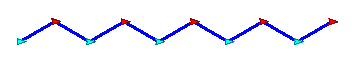
\includegraphics[width=0.75\textwidth]{figs/bad-hexagon}
    \end{minipage}
    \begin{minipage}[b]{0.95\linewidth}
        \centering
        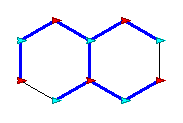
\includegraphics[width=0.3\textwidth]{figs/good-hexagon}
    \end{minipage}
    \caption{Possible formations of $10$ robots satisfying the hexagon lattice graph (Figure~\ref{fig:hex}). 
    [top] Fulfillment ratio $\Quality=0.6$. 
    [bottom] Fulfillment ratio $\Quality = 0.733$.}
    \label{fig:hex-qual}
\end{figure}

\subsubsection{Formation Fulfillment Ratio}

The second measurement is the quality of the finally formed pattern.
%
When all robots reach static positions, for robot $r_i$
with $E_i$ outgoing edges from its role vertex, 
namely, the maximum number of neighbors it could have in order to form the desired lattice represented by given lattice graph. 
If the actual number of neighbors it has is $N_i$, 
we evaluate the overall lattice quality by a fulfillment ratio:
\begin{equation}\label{eq:gamma}
  \Quality = \dfrac{1}{n}\sum\limits_{i=1}^n \frac{N_i}{E_i}
\end{equation}

The ratio $\Quality \in [0, 1]$ approximately reflects how satisfactory the final formation is 
with regard to the given lattice graph. 
%
We prefer a formation with a value of $\Quality$ as large as possible.

Figure~\ref{fig:hex-qual} shows that both sets of robots satisfy the lattice
graph in Figure~\ref{fig:hex} but with different fulfillment ratios.


